\documentclass[Main.tex]{subfiles}
\begin{document}
	\hienthiloigiaibt
	\hienthiloigiaiex
	\begin{bt}
		\immini{Vẽ lại hình vẽ bên và tô màu để phân số biểu thị phần tô màu bằng $\dfrac{5}{12}$
		}{
			\resizebox{4cm}{!}{
\begin{tikzpicture}
				\draw (0,0) grid (4,-3);
			\end{tikzpicture}}
		}
		\loigiai{Ta cần tô $5$ ô trong $12$ ô của hình
			\begin{center}
				\resizebox{4cm}{!}{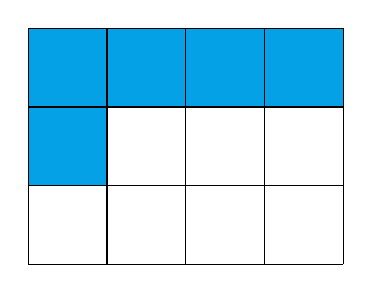
\begin{tikzpicture}
						\fill[cyan!90!blue] (0,0) rectangle (4,-1)
						(0,-1) rectangle (1,-2);
						\draw (0,0) grid (4,-3);
				\end{tikzpicture}}
			\end{center}
		}
	\end{bt}
	
	\medskip
	\Opensolutionfile{ans}[Ans/DapanChuong]
	\begin{ex}
		\renewcommand{\dotEX}{}
		Chọn hình vẽ có phần tô màu biểu thị phân số $\dfrac{5}{12}$
		\choice
		{\True
			\resizebox{4cm}{!}{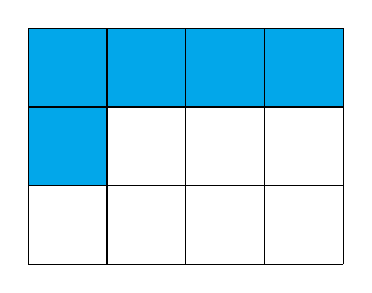
\begin{tikzpicture}
					\fill[cyan!95!blue] (0,0) rectangle (4,-1)
					(0,-1) rectangle (1,-2);
					\draw (0,0) grid (4,-3);
			\end{tikzpicture}}
		}
		{\resizebox{4cm}{!}{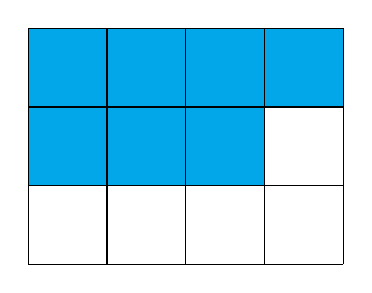
\begin{tikzpicture}
					\fill[cyan!95!blue] (0,0) rectangle (4,-1)
					(0,-1) rectangle (3,-2);
					\draw (0,0) grid (4,-3);
			\end{tikzpicture}}
		}
		{\resizebox{4cm}{!}{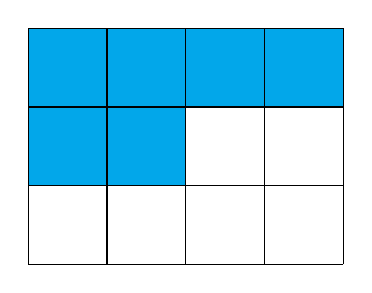
\begin{tikzpicture}
					\fill[cyan!95!blue] (0,0) rectangle (4,-1)
					(0,-1) rectangle (2,-2);
					\draw (0,0) grid (4,-3);
			\end{tikzpicture}}
		}
		{\resizebox{4cm}{!}{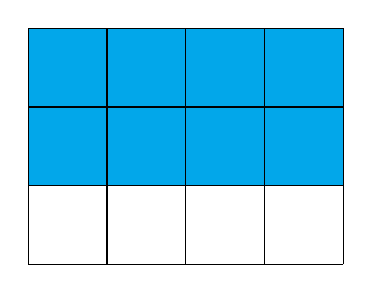
\begin{tikzpicture}
					\fill[cyan!95!blue] (0,0) rectangle (4,-2);
					\draw (0,0) grid (4,-3);
			\end{tikzpicture}}
		} 	 	
		\loigiai{
			Hình vẽ đúng là hình có tô $5$ ô trong $12$ ô.
		}
	\end{ex}
	\Closesolutionfile{ans}
	
	
	\Opensolutionfile{ans}[Ans/DapanChuong]
	\Opensolutionfile{ansbook}[Ansbook/DapanTFChuong]
	\begin{ex}
		Cho biểu thức $A=\dfrac{-2}{3}-\left(\dfrac{m}{n}+\dfrac{-5}{2}\right)\cdot\dfrac{-5}{8}\cdot$
		\choiceTF
		{\True }
		{}
		{\True}
		{}
		\loigiai{
			Ta có 
			\begin{align*}
				A &=\dfrac{-2}{3}-\left(\dfrac{m}{n}+\dfrac{-5}{2}\right)\cdot\dfrac{-5}{8}\\
				&=\dfrac{-2}{3}+\dfrac{5m}{8n}-\dfrac{25}{16}\\
				&=\dfrac{5m}{8n}+\dfrac{-2}{3}-\dfrac{25}{16}\\
				&=\dfrac{5m}{8n}-\dfrac{107}{48}
			\end{align*}
			\begin{itemize}
				\item 
				\item 
				\item 
				\item 
			\end{itemize}
		}
	\end{ex}
	\Closesolutionfile{ans}
	\Closesolutionfile{ansbook}
\end{document}